\definecolor{r1}{RGB}{86,16,16};
\definecolor{r2}{RGB}{151,28,28};
\definecolor{r3}{RGB}{214,39,40};
\definecolor{r4}{RGB}{227,104,104};
\definecolor{r5}{RGB}{239,169,169};
\definecolor{b1}{RGB}{11,43,65};
\definecolor{b2}{RGB}{22,86,131};
\definecolor{b3}{RGB}{31,119,180};
\definecolor{b4}{RGB}{59,154,222};
\definecolor{b5}{RGB}{124,188,233};
\definecolor{g1}{RGB}{16,60,16};
\definecolor{g2}{RGB}{33,120,33};
\definecolor{g3}{RGB}{49,180,49};
\definecolor{g4}{RGB}{95,211,95};
\definecolor{g5}{RGB}{135,222,135};
\definecolor{p1}{RGB}{39,23,53};
\definecolor{p2}{RGB}{77,47,106};
\definecolor{p3}{RGB}{116,70,160};
\definecolor{p4}{RGB}{148,103,189};
\definecolor{p5}{RGB}{179,149,208};
\definecolor{tab_orange}{RGB}{255,127,14};
\definecolor{tab_blue}{RGB}{31, 119, 180};
\definecolor{mixed_color}{RGB}{143, 123, 97}
\definecolor{tab_brown}{RGB}{140,86,75};


\begin{tikzpicture}

\node at (-0.2,12.7) {{\fontfamily{phv}\scalebox{1}{\fontsize{8pt}{0pt}\selectfont{A}}}};

\node at (2.6,12.7) {{\fontfamily{phv}\scalebox{1}{\fontsize{7pt}{0pt}\selectfont \parbox{4.5cm} {\hyphenpenalty=10000\exhyphenpenalty=10000\raggedright
Positive and Negative Syndrome Scale scores
}}}};
\node[inner sep=0pt] (russell) at (2.4,9.7) {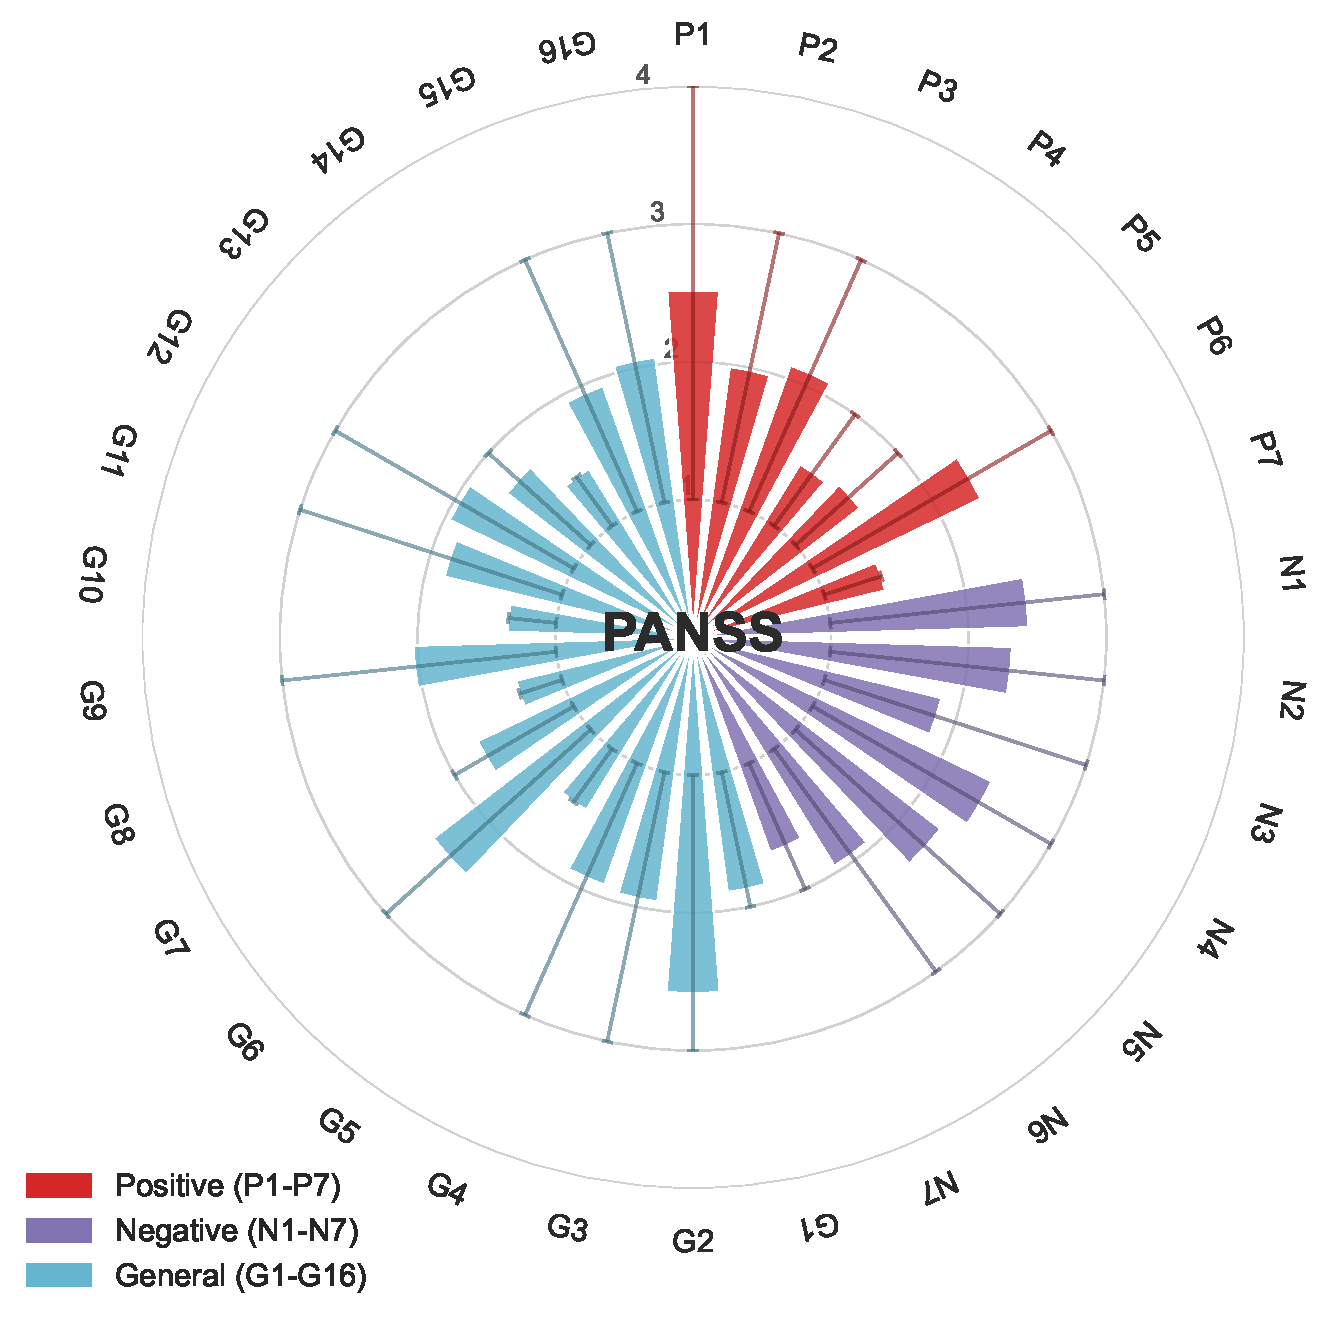
\includegraphics[width=0.25\textwidth]{figB1.pdf}};


\node at (5.3,12.7) {{\fontfamily{phv}\scalebox{1}{\fontsize{8pt}{0pt}\selectfont{B}}}};

\node at (8.1,12.7) {{\fontfamily{phv}\scalebox{1}{\fontsize{7pt}{0pt}\selectfont \parbox{4.5cm} {\hyphenpenalty=10000\exhyphenpenalty=10000\raggedright
Hamilton Depression Rating Scale scores
}}}};
\node[inner sep=0pt] (russell) at (7.9,9.7) {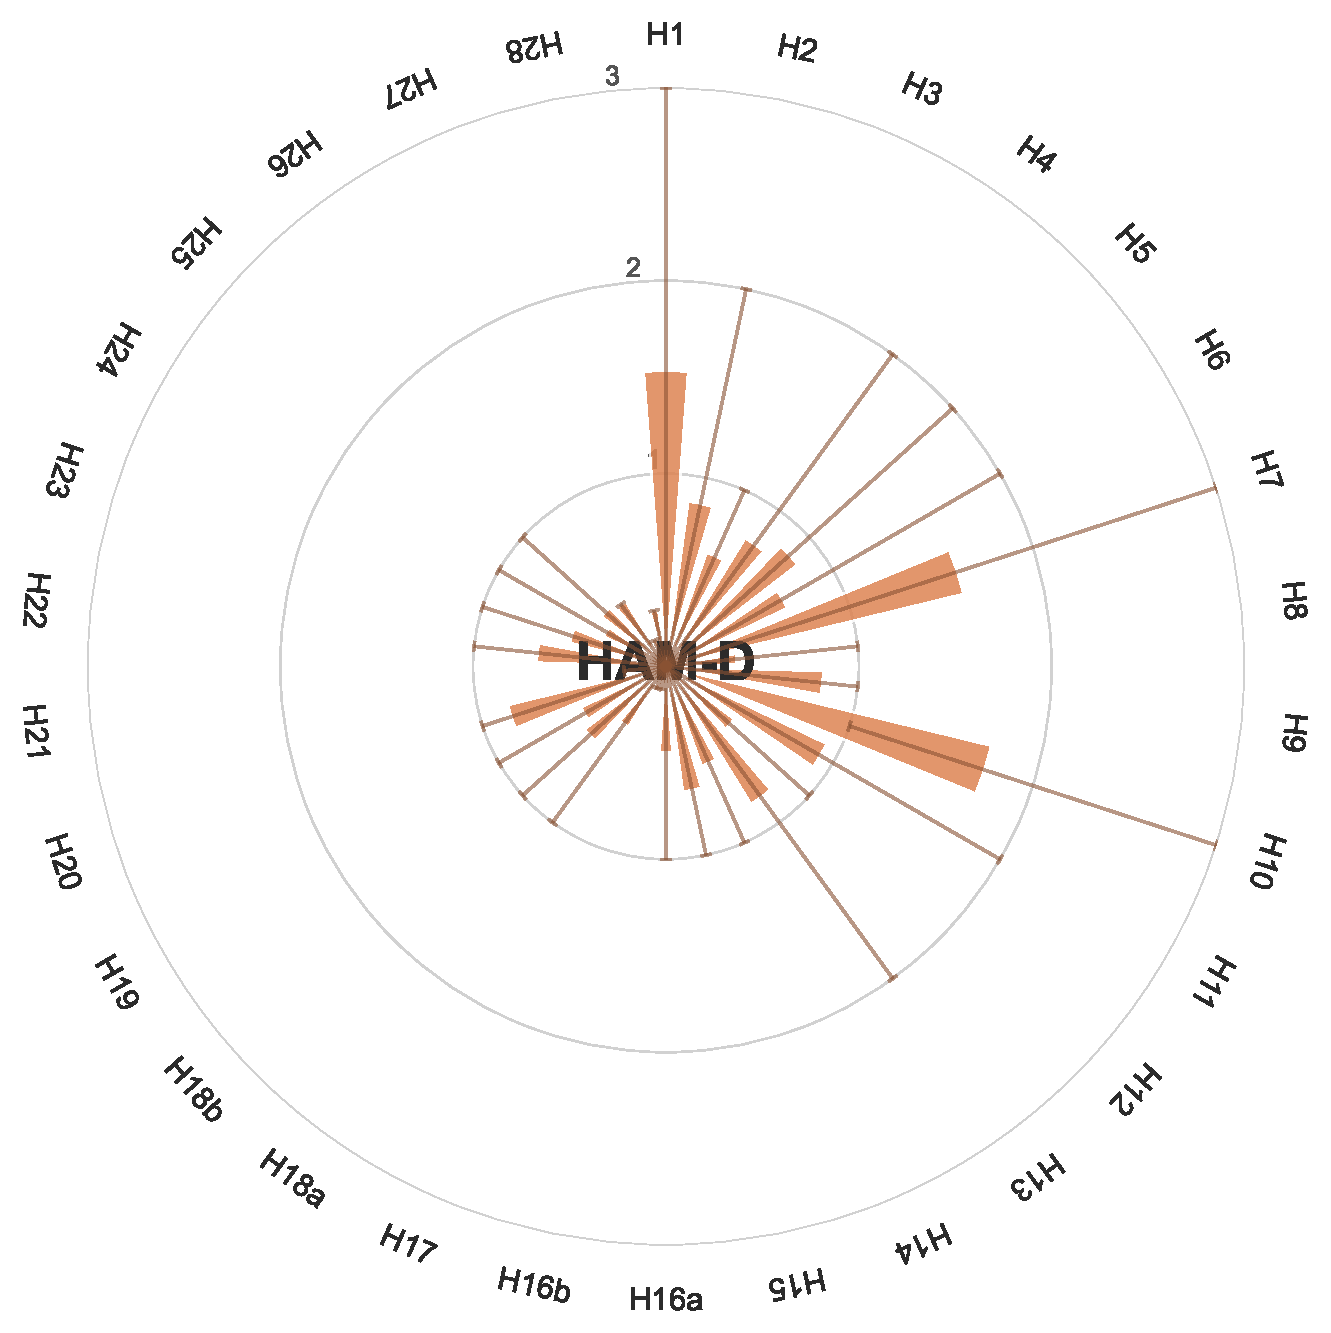
\includegraphics[width=0.25\textwidth]{figB2.pdf}};

\node at (-0.2,6.4) {{\fontfamily{phv}\scalebox{1}{\fontsize{8pt}{0pt}\selectfont{C}}}};

\node at (2.6,6.4) {{\fontfamily{phv}\scalebox{1}{\fontsize{7pt}{0pt}\selectfont \parbox{4.5cm} {\hyphenpenalty=10000\exhyphenpenalty=10000\raggedright
Scale for the Assessment of Negative Symptoms scores
}}}};
\node[inner sep=0pt] (russell) at (2.4,3.4) {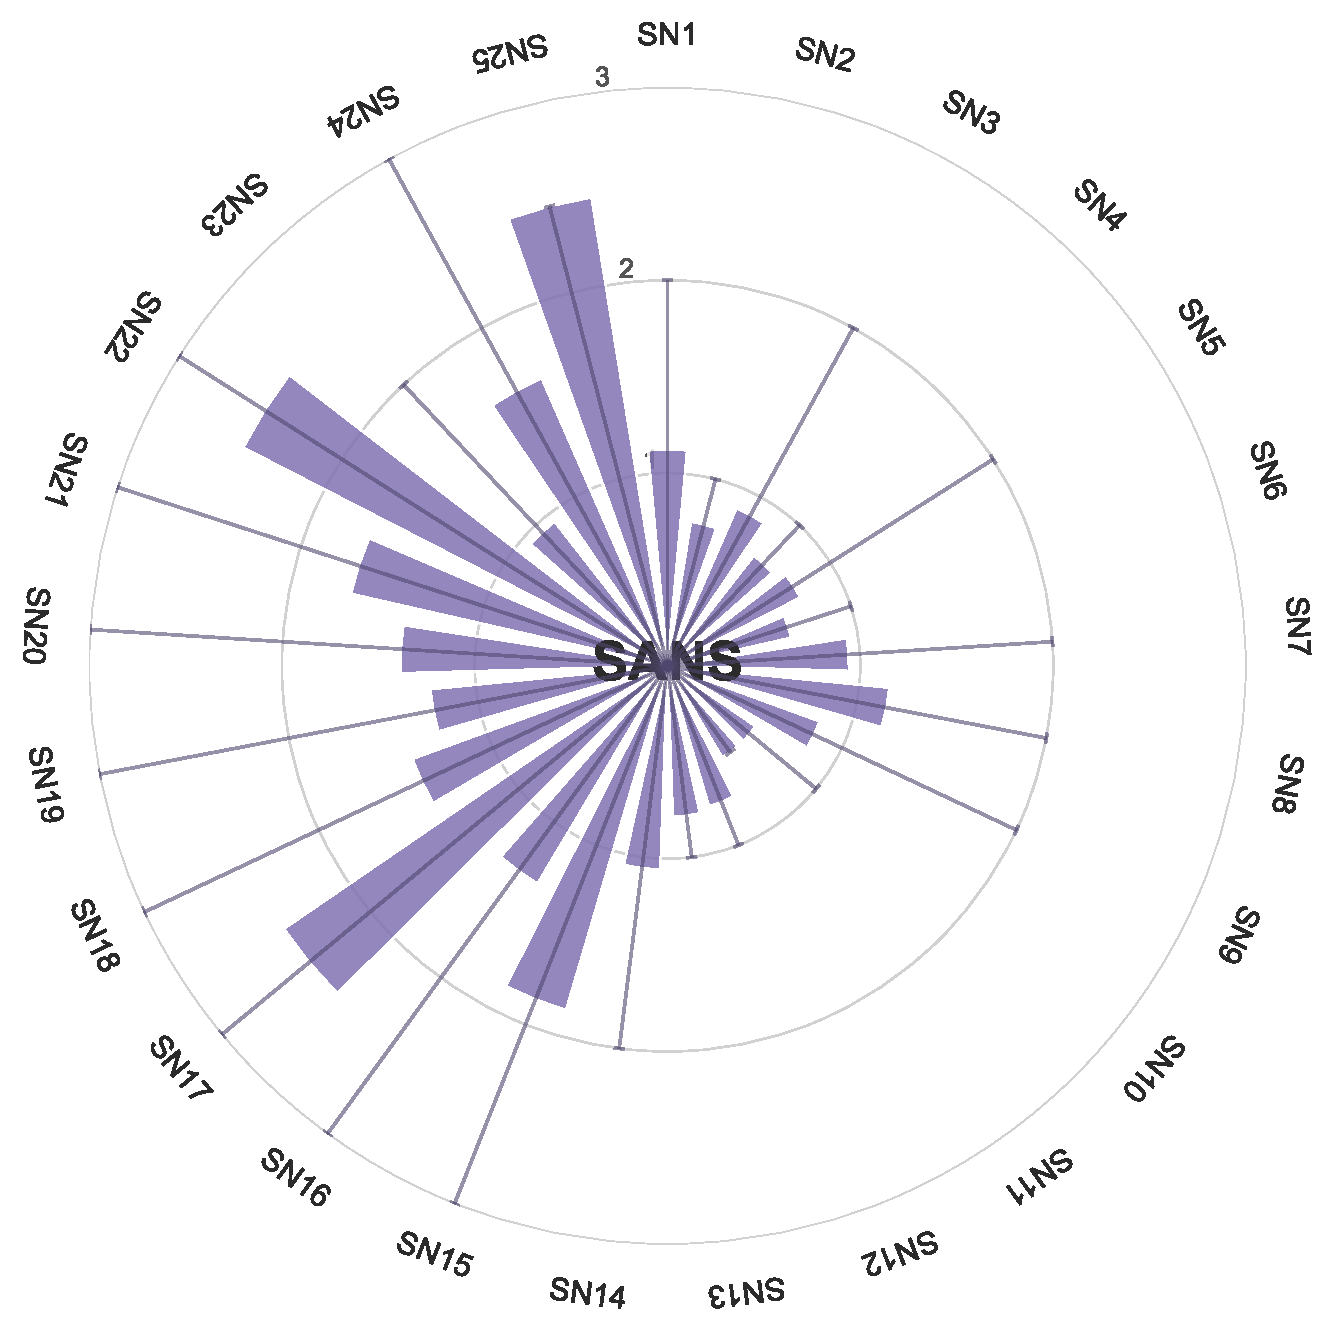
\includegraphics[width=0.25\textwidth]{figB3.pdf}};



\node at (5.3,6.4) {{\fontfamily{phv}\scalebox{1}{\fontsize{8pt}{0pt}\selectfont{D}}}};

\node at (8.1,6.4) {{\fontfamily{phv}\scalebox{1}{\fontsize{7pt}{0pt}\selectfont \parbox{4.5cm} {\hyphenpenalty=10000\exhyphenpenalty=10000\raggedright
Scale for the Assessment of Positive Symptoms
}}}};
\node[inner sep=0pt] (russell) at (7.9,3.4) {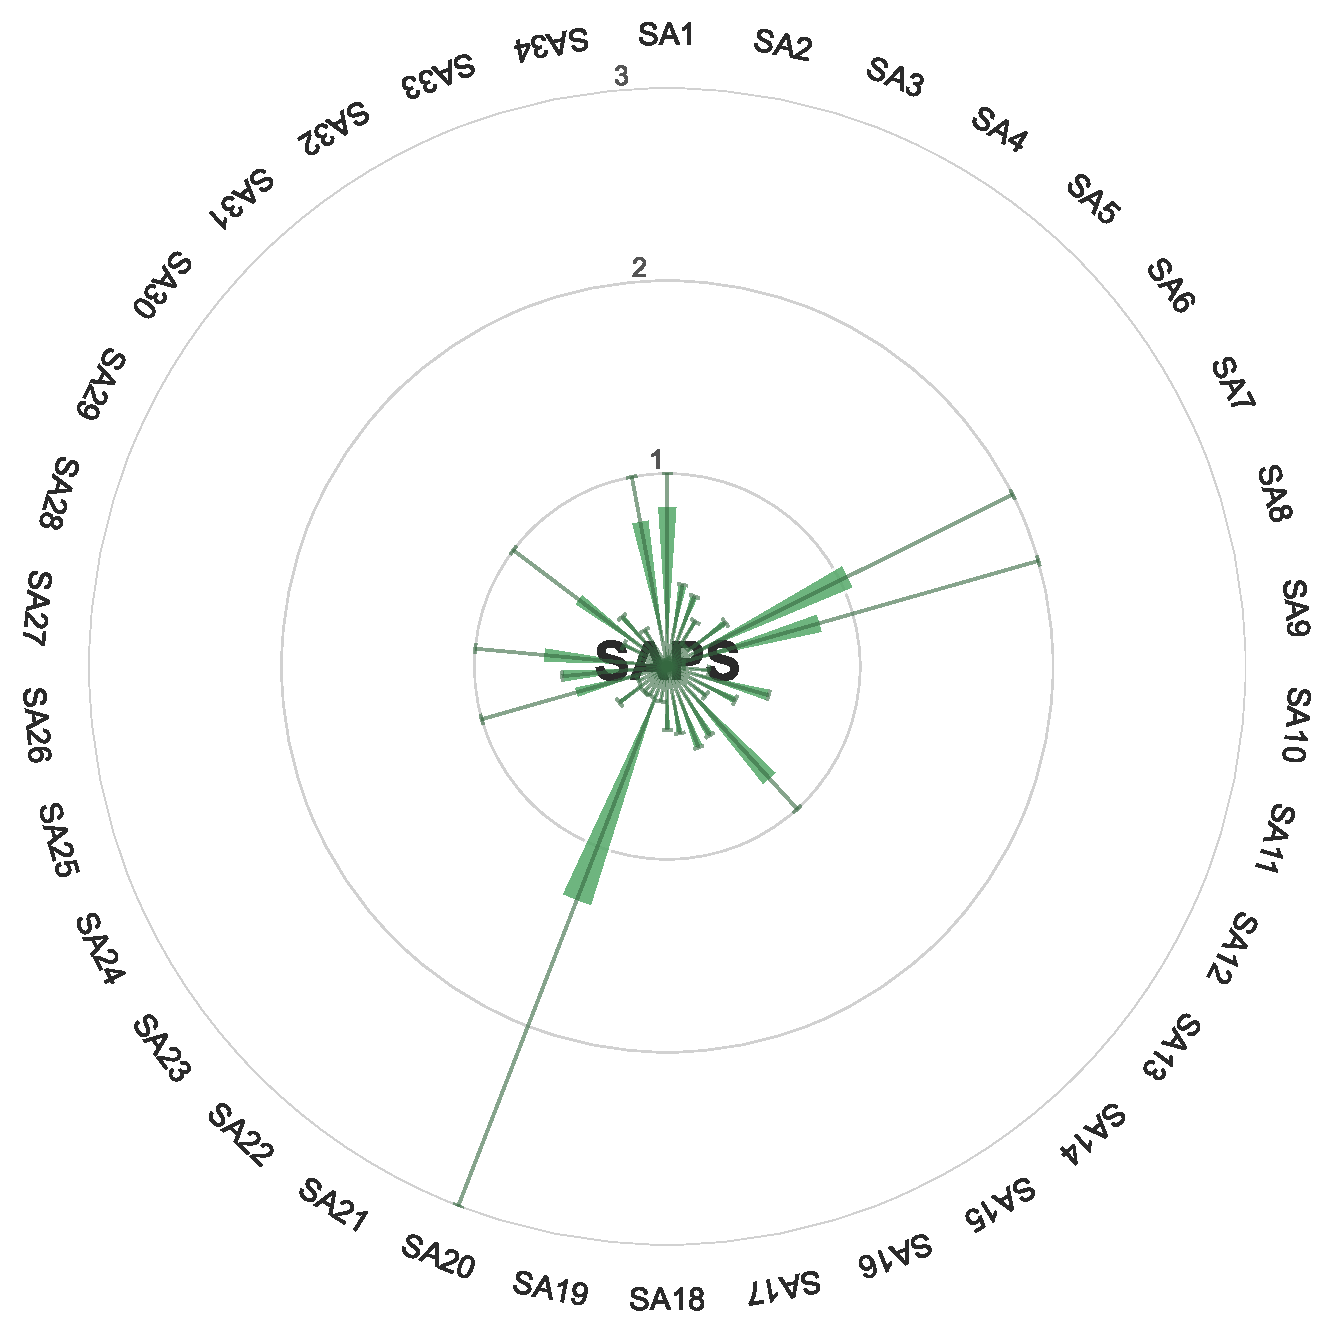
\includegraphics[width=0.25\textwidth]{figB4.pdf}};























% Panel A caption line (place under figB1 image)
\node at (2.8,8) {{\fontfamily{phv}\scalebox{1}{\fontsize{4pt}{0pt}\selectfont \parbox{2cm} {\raggedright
Available for 699 participants (7.8\% of databank): SSD 30.5\% (423/1,387), HC 1.6\% (81/5,071), MDD 5.7\% (45/786)
}}}};

% Panel B caption line (place under figB2 image)
\node at (8.3,8) {{\fontfamily{phv}\scalebox{1}{\fontsize{4pt}{0pt}\selectfont \parbox{2cm} {\raggedright
Available for 212 participants (2.4\% of databank): MDD 8.9\% (70/786), SSD 3.6\% (50/1,387), BD 20.2\% (49/243)
}}}};

% Panel C caption line (place under figB3 image)
\node at (2.8,1.7) {{\fontfamily{phv}\scalebox{1}{\fontsize{4pt}{0pt}\selectfont \parbox{2cm} {\raggedright
Available for 810 participants (9.0\% of databank): SSD 38.9\% (539/1,387), HC 1.6\% (80/5,071)
}}}};

% Panel D caption line (place under figB4 image)
\node at (8.3,1.7) {{\fontfamily{phv}\scalebox{1}{\fontsize{4pt}{0pt}\selectfont \parbox{2cm} {\raggedright
Available for 605 participants (6.7\% of databank): SSD 24.2\% (335/1,387), HC 1.6\% (80/5,071)
}}}};


\end{tikzpicture}